\documentclass[11pt]{article}
\usepackage{sectsty}
\allsectionsfont{\color{blue}\fontfamily{lmss}\selectfont}
\usepackage{fontspec}
\setmainfont{XCharter}

\usepackage{listings}
\lstset{
basicstyle=\small\ttfamily,
tabsize=8,
columns=flexible,
breaklines=true,
frame=tb,
rulecolor=\color[rgb]{0.8,0.8,0.7},
backgroundcolor=\color[rgb]{1,1,0.91},
postbreak=\raisebox{0ex}[0ex][0ex]{\ensuremath{\color{red}\hookrightarrow\space}}
}
\usepackage{fontawesome}


\usepackage{mdframed}
\newmdenv[
  backgroundcolor=gray,
  fontcolor=white,
  nobreak=true,
]{terminalinput}



\usepackage{parskip}


    \usepackage[breakable]{tcolorbox}
    \usepackage{parskip} % Stop auto-indenting (to mimic markdown behaviour)

    \usepackage{iftex}
    \ifPDFTeX
    	\usepackage[T1]{fontenc}
    	\usepackage{mathpazo}
    \else
    	\usepackage{fontspec}
    \fi

    % Basic figure setup, for now with no caption control since it's done
    % automatically by Pandoc (which extracts ![](path) syntax from Markdown).
    \usepackage{graphicx}
    % Maintain compatibility with old templates. Remove in nbconvert 6.0
    \let\Oldincludegraphics\includegraphics
    % Ensure that by default, figures have no caption (until we provide a
    % proper Figure object with a Caption API and a way to capture that
    % in the conversion process - todo).
    \usepackage{caption}
    \DeclareCaptionFormat{nocaption}{}
    \captionsetup{format=nocaption,aboveskip=0pt,belowskip=0pt}

    \usepackage[Export]{adjustbox} % Used to constrain images to a maximum size
    \adjustboxset{max size={0.9\linewidth}{0.9\paperheight}}
    \usepackage{float}
    \floatplacement{figure}{H} % forces figures to be placed at the correct location
    \usepackage{xcolor} % Allow colors to be defined
    \usepackage{enumerate} % Needed for markdown enumerations to work
    \usepackage{geometry} % Used to adjust the document margins
    \usepackage{amsmath} % Equations
    \usepackage{amssymb} % Equations
    \usepackage{textcomp} % defines textquotesingle
    % Hack from http://tex.stackexchange.com/a/47451/13684:
    \AtBeginDocument{%
        \def\PYZsq{\textquotesingle}% Upright quotes in Pygmentized code
    }
    \usepackage{upquote} % Upright quotes for verbatim code
    \usepackage{eurosym} % defines \euro
    \usepackage[mathletters]{ucs} % Extended unicode (utf-8) support
    \usepackage{fancyvrb} % verbatim replacement that allows latex
    \usepackage{grffile} % extends the file name processing of package graphics
                         % to support a larger range
    \makeatletter % fix for grffile with XeLaTeX
    \def\Gread@@xetex#1{%
      \IfFileExists{"\Gin@base".bb}%
      {\Gread@eps{\Gin@base.bb}}%
      {\Gread@@xetex@aux#1}%
    }
    \makeatother

    % The hyperref package gives us a pdf with properly built
    % internal navigation ('pdf bookmarks' for the table of contents,
    % internal cross-reference links, web links for URLs, etc.)
    \usepackage{hyperref}
    % The default LaTeX title has an obnoxious amount of whitespace. By default,
    % titling removes some of it. It also provides customization options.
    \usepackage{titling}
    \usepackage{longtable} % longtable support required by pandoc >1.10
    \usepackage{booktabs}  % table support for pandoc > 1.12.2
    \usepackage[inline]{enumitem} % IRkernel/repr support (it uses the enumerate* environment)
    \usepackage[normalem]{ulem} % ulem is needed to support strikethroughs (\sout)
                                % normalem makes italics be italics, not underlines
    \usepackage{mathrsfs}



    % Colors for the hyperref package
    \definecolor{urlcolor}{rgb}{0,.145,.698}
    \definecolor{linkcolor}{rgb}{.71,0.21,0.01}
    \definecolor{citecolor}{rgb}{.12,.54,.11}

    % ANSI colors
    \definecolor{ansi-black}{HTML}{3E424D}
    \definecolor{ansi-black-intense}{HTML}{282C36}
    \definecolor{ansi-red}{HTML}{E75C58}
    \definecolor{ansi-red-intense}{HTML}{B22B31}
    \definecolor{ansi-green}{HTML}{00A250}
    \definecolor{ansi-green-intense}{HTML}{007427}
    \definecolor{ansi-yellow}{HTML}{DDB62B}
    \definecolor{ansi-yellow-intense}{HTML}{B27D12}
    \definecolor{ansi-blue}{HTML}{208FFB}
    \definecolor{ansi-blue-intense}{HTML}{0065CA}
    \definecolor{ansi-magenta}{HTML}{D160C4}
    \definecolor{ansi-magenta-intense}{HTML}{A03196}
    \definecolor{ansi-cyan}{HTML}{60C6C8}
    \definecolor{ansi-cyan-intense}{HTML}{258F8F}
    \definecolor{ansi-white}{HTML}{C5C1B4}
    \definecolor{ansi-white-intense}{HTML}{A1A6B2}
    \definecolor{ansi-default-inverse-fg}{HTML}{FFFFFF}
    \definecolor{ansi-default-inverse-bg}{HTML}{000000}

    % commands and environments needed by pandoc snippets
    % extracted from the output of `pandoc -s`
    \providecommand{\tightlist}{%
      \setlength{\itemsep}{0pt}\setlength{\parskip}{0pt}}
    \DefineVerbatimEnvironment{Highlighting}{Verbatim}{commandchars=\\\{\}}
    % Add ',fontsize=\small' for more characters per line
    \newenvironment{Shaded}{}{}
    \newcommand{\KeywordTok}[1]{\textcolor[rgb]{0.00,0.44,0.13}{\textbf{{#1}}}}
    \newcommand{\DataTypeTok}[1]{\textcolor[rgb]{0.56,0.13,0.00}{{#1}}}
    \newcommand{\DecValTok}[1]{\textcolor[rgb]{0.25,0.63,0.44}{{#1}}}
    \newcommand{\BaseNTok}[1]{\textcolor[rgb]{0.25,0.63,0.44}{{#1}}}
    \newcommand{\FloatTok}[1]{\textcolor[rgb]{0.25,0.63,0.44}{{#1}}}
    \newcommand{\CharTok}[1]{\textcolor[rgb]{0.25,0.44,0.63}{{#1}}}
    \newcommand{\StringTok}[1]{\textcolor[rgb]{0.25,0.44,0.63}{{#1}}}
    \newcommand{\CommentTok}[1]{\textcolor[rgb]{0.38,0.63,0.69}{\textit{{#1}}}}
    \newcommand{\OtherTok}[1]{\textcolor[rgb]{0.00,0.44,0.13}{{#1}}}
    \newcommand{\AlertTok}[1]{\textcolor[rgb]{1.00,0.00,0.00}{\textbf{{#1}}}}
    \newcommand{\FunctionTok}[1]{\textcolor[rgb]{0.02,0.16,0.49}{{#1}}}
    \newcommand{\RegionMarkerTok}[1]{{#1}}
    \newcommand{\ErrorTok}[1]{\textcolor[rgb]{1.00,0.00,0.00}{\textbf{{#1}}}}
    \newcommand{\NormalTok}[1]{{#1}}

    % Additional commands for more recent versions of Pandoc
    \newcommand{\ConstantTok}[1]{\textcolor[rgb]{0.53,0.00,0.00}{{#1}}}
    \newcommand{\SpecialCharTok}[1]{\textcolor[rgb]{0.25,0.44,0.63}{{#1}}}
    \newcommand{\VerbatimStringTok}[1]{\textcolor[rgb]{0.25,0.44,0.63}{{#1}}}
    \newcommand{\SpecialStringTok}[1]{\textcolor[rgb]{0.73,0.40,0.53}{{#1}}}
    \newcommand{\ImportTok}[1]{{#1}}
    \newcommand{\DocumentationTok}[1]{\textcolor[rgb]{0.73,0.13,0.13}{\textit{{#1}}}}
    \newcommand{\AnnotationTok}[1]{\textcolor[rgb]{0.38,0.63,0.69}{\textbf{\textit{{#1}}}}}
    \newcommand{\CommentVarTok}[1]{\textcolor[rgb]{0.38,0.63,0.69}{\textbf{\textit{{#1}}}}}
    \newcommand{\VariableTok}[1]{\textcolor[rgb]{0.10,0.09,0.49}{{#1}}}
    \newcommand{\ControlFlowTok}[1]{\textcolor[rgb]{0.00,0.44,0.13}{\textbf{{#1}}}}
    \newcommand{\OperatorTok}[1]{\textcolor[rgb]{0.40,0.40,0.40}{{#1}}}
    \newcommand{\BuiltInTok}[1]{{#1}}
    \newcommand{\ExtensionTok}[1]{{#1}}
    \newcommand{\PreprocessorTok}[1]{\textcolor[rgb]{0.74,0.48,0.00}{{#1}}}
    \newcommand{\AttributeTok}[1]{\textcolor[rgb]{0.49,0.56,0.16}{{#1}}}
    \newcommand{\InformationTok}[1]{\textcolor[rgb]{0.38,0.63,0.69}{\textbf{\textit{{#1}}}}}
    \newcommand{\WarningTok}[1]{\textcolor[rgb]{0.38,0.63,0.69}{\textbf{\textit{{#1}}}}}


    % Define a nice break command that doesn't care if a line doesn't already
    % exist.
    \def\br{\hspace*{\fill} \\* }
    % Math Jax compatibility definitions
    \def\gt{>}
    \def\lt{<}
    \let\Oldtex\TeX
    \let\Oldlatex\LaTeX
    \renewcommand{\TeX}{\textrm{\Oldtex}}
    \renewcommand{\LaTeX}{\textrm{\Oldlatex}}
    % Document parameters
    % Document title
    \title{index}





% Pygments definitions
\makeatletter
\def\PY@reset{\let\PY@it=\relax \let\PY@bf=\relax%
    \let\PY@ul=\relax \let\PY@tc=\relax%
    \let\PY@bc=\relax \let\PY@ff=\relax}
\def\PY@tok#1{\csname PY@tok@#1\endcsname}
\def\PY@toks#1+{\ifx\relax#1\empty\else%
    \PY@tok{#1}\expandafter\PY@toks\fi}
\def\PY@do#1{\PY@bc{\PY@tc{\PY@ul{%
    \PY@it{\PY@bf{\PY@ff{#1}}}}}}}
\def\PY#1#2{\PY@reset\PY@toks#1+\relax+\PY@do{#2}}

\expandafter\def\csname PY@tok@w\endcsname{\def\PY@tc##1{\textcolor[rgb]{0.73,0.73,0.73}{##1}}}
\expandafter\def\csname PY@tok@c\endcsname{\let\PY@it=\textit\def\PY@tc##1{\textcolor[rgb]{0.25,0.50,0.50}{##1}}}
\expandafter\def\csname PY@tok@cp\endcsname{\def\PY@tc##1{\textcolor[rgb]{0.74,0.48,0.00}{##1}}}
\expandafter\def\csname PY@tok@k\endcsname{\let\PY@bf=\textbf\def\PY@tc##1{\textcolor[rgb]{0.00,0.50,0.00}{##1}}}
\expandafter\def\csname PY@tok@kp\endcsname{\def\PY@tc##1{\textcolor[rgb]{0.00,0.50,0.00}{##1}}}
\expandafter\def\csname PY@tok@kt\endcsname{\def\PY@tc##1{\textcolor[rgb]{0.69,0.00,0.25}{##1}}}
\expandafter\def\csname PY@tok@o\endcsname{\def\PY@tc##1{\textcolor[rgb]{0.40,0.40,0.40}{##1}}}
\expandafter\def\csname PY@tok@ow\endcsname{\let\PY@bf=\textbf\def\PY@tc##1{\textcolor[rgb]{0.67,0.13,1.00}{##1}}}
\expandafter\def\csname PY@tok@nb\endcsname{\def\PY@tc##1{\textcolor[rgb]{0.00,0.50,0.00}{##1}}}
\expandafter\def\csname PY@tok@nf\endcsname{\def\PY@tc##1{\textcolor[rgb]{0.00,0.00,1.00}{##1}}}
\expandafter\def\csname PY@tok@nc\endcsname{\let\PY@bf=\textbf\def\PY@tc##1{\textcolor[rgb]{0.00,0.00,1.00}{##1}}}
\expandafter\def\csname PY@tok@nn\endcsname{\let\PY@bf=\textbf\def\PY@tc##1{\textcolor[rgb]{0.00,0.00,1.00}{##1}}}
\expandafter\def\csname PY@tok@ne\endcsname{\let\PY@bf=\textbf\def\PY@tc##1{\textcolor[rgb]{0.82,0.25,0.23}{##1}}}
\expandafter\def\csname PY@tok@nv\endcsname{\def\PY@tc##1{\textcolor[rgb]{0.10,0.09,0.49}{##1}}}
\expandafter\def\csname PY@tok@no\endcsname{\def\PY@tc##1{\textcolor[rgb]{0.53,0.00,0.00}{##1}}}
\expandafter\def\csname PY@tok@nl\endcsname{\def\PY@tc##1{\textcolor[rgb]{0.63,0.63,0.00}{##1}}}
\expandafter\def\csname PY@tok@ni\endcsname{\let\PY@bf=\textbf\def\PY@tc##1{\textcolor[rgb]{0.60,0.60,0.60}{##1}}}
\expandafter\def\csname PY@tok@na\endcsname{\def\PY@tc##1{\textcolor[rgb]{0.49,0.56,0.16}{##1}}}
\expandafter\def\csname PY@tok@nt\endcsname{\let\PY@bf=\textbf\def\PY@tc##1{\textcolor[rgb]{0.00,0.50,0.00}{##1}}}
\expandafter\def\csname PY@tok@nd\endcsname{\def\PY@tc##1{\textcolor[rgb]{0.67,0.13,1.00}{##1}}}
\expandafter\def\csname PY@tok@s\endcsname{\def\PY@tc##1{\textcolor[rgb]{0.73,0.13,0.13}{##1}}}
\expandafter\def\csname PY@tok@sd\endcsname{\let\PY@it=\textit\def\PY@tc##1{\textcolor[rgb]{0.73,0.13,0.13}{##1}}}
\expandafter\def\csname PY@tok@si\endcsname{\let\PY@bf=\textbf\def\PY@tc##1{\textcolor[rgb]{0.73,0.40,0.53}{##1}}}
\expandafter\def\csname PY@tok@se\endcsname{\let\PY@bf=\textbf\def\PY@tc##1{\textcolor[rgb]{0.73,0.40,0.13}{##1}}}
\expandafter\def\csname PY@tok@sr\endcsname{\def\PY@tc##1{\textcolor[rgb]{0.73,0.40,0.53}{##1}}}
\expandafter\def\csname PY@tok@ss\endcsname{\def\PY@tc##1{\textcolor[rgb]{0.10,0.09,0.49}{##1}}}
\expandafter\def\csname PY@tok@sx\endcsname{\def\PY@tc##1{\textcolor[rgb]{0.00,0.50,0.00}{##1}}}
\expandafter\def\csname PY@tok@m\endcsname{\def\PY@tc##1{\textcolor[rgb]{0.40,0.40,0.40}{##1}}}
\expandafter\def\csname PY@tok@gh\endcsname{\let\PY@bf=\textbf\def\PY@tc##1{\textcolor[rgb]{0.00,0.00,0.50}{##1}}}
\expandafter\def\csname PY@tok@gu\endcsname{\let\PY@bf=\textbf\def\PY@tc##1{\textcolor[rgb]{0.50,0.00,0.50}{##1}}}
\expandafter\def\csname PY@tok@gd\endcsname{\def\PY@tc##1{\textcolor[rgb]{0.63,0.00,0.00}{##1}}}
\expandafter\def\csname PY@tok@gi\endcsname{\def\PY@tc##1{\textcolor[rgb]{0.00,0.63,0.00}{##1}}}
\expandafter\def\csname PY@tok@gr\endcsname{\def\PY@tc##1{\textcolor[rgb]{1.00,0.00,0.00}{##1}}}
\expandafter\def\csname PY@tok@ge\endcsname{\let\PY@it=\textit}
\expandafter\def\csname PY@tok@gs\endcsname{\let\PY@bf=\textbf}
\expandafter\def\csname PY@tok@gp\endcsname{\let\PY@bf=\textbf\def\PY@tc##1{\textcolor[rgb]{0.00,0.00,0.50}{##1}}}
\expandafter\def\csname PY@tok@go\endcsname{\def\PY@tc##1{\textcolor[rgb]{0.53,0.53,0.53}{##1}}}
\expandafter\def\csname PY@tok@gt\endcsname{\def\PY@tc##1{\textcolor[rgb]{0.00,0.27,0.87}{##1}}}
\expandafter\def\csname PY@tok@err\endcsname{\def\PY@bc##1{\setlength{\fboxsep}{0pt}\fcolorbox[rgb]{1.00,0.00,0.00}{1,1,1}{\strut ##1}}}
\expandafter\def\csname PY@tok@kc\endcsname{\let\PY@bf=\textbf\def\PY@tc##1{\textcolor[rgb]{0.00,0.50,0.00}{##1}}}
\expandafter\def\csname PY@tok@kd\endcsname{\let\PY@bf=\textbf\def\PY@tc##1{\textcolor[rgb]{0.00,0.50,0.00}{##1}}}
\expandafter\def\csname PY@tok@kn\endcsname{\let\PY@bf=\textbf\def\PY@tc##1{\textcolor[rgb]{0.00,0.50,0.00}{##1}}}
\expandafter\def\csname PY@tok@kr\endcsname{\let\PY@bf=\textbf\def\PY@tc##1{\textcolor[rgb]{0.00,0.50,0.00}{##1}}}
\expandafter\def\csname PY@tok@bp\endcsname{\def\PY@tc##1{\textcolor[rgb]{0.00,0.50,0.00}{##1}}}
\expandafter\def\csname PY@tok@fm\endcsname{\def\PY@tc##1{\textcolor[rgb]{0.00,0.00,1.00}{##1}}}
\expandafter\def\csname PY@tok@vc\endcsname{\def\PY@tc##1{\textcolor[rgb]{0.10,0.09,0.49}{##1}}}
\expandafter\def\csname PY@tok@vg\endcsname{\def\PY@tc##1{\textcolor[rgb]{0.10,0.09,0.49}{##1}}}
\expandafter\def\csname PY@tok@vi\endcsname{\def\PY@tc##1{\textcolor[rgb]{0.10,0.09,0.49}{##1}}}
\expandafter\def\csname PY@tok@vm\endcsname{\def\PY@tc##1{\textcolor[rgb]{0.10,0.09,0.49}{##1}}}
\expandafter\def\csname PY@tok@sa\endcsname{\def\PY@tc##1{\textcolor[rgb]{0.73,0.13,0.13}{##1}}}
\expandafter\def\csname PY@tok@sb\endcsname{\def\PY@tc##1{\textcolor[rgb]{0.73,0.13,0.13}{##1}}}
\expandafter\def\csname PY@tok@sc\endcsname{\def\PY@tc##1{\textcolor[rgb]{0.73,0.13,0.13}{##1}}}
\expandafter\def\csname PY@tok@dl\endcsname{\def\PY@tc##1{\textcolor[rgb]{0.73,0.13,0.13}{##1}}}
\expandafter\def\csname PY@tok@s2\endcsname{\def\PY@tc##1{\textcolor[rgb]{0.73,0.13,0.13}{##1}}}
\expandafter\def\csname PY@tok@sh\endcsname{\def\PY@tc##1{\textcolor[rgb]{0.73,0.13,0.13}{##1}}}
\expandafter\def\csname PY@tok@s1\endcsname{\def\PY@tc##1{\textcolor[rgb]{0.73,0.13,0.13}{##1}}}
\expandafter\def\csname PY@tok@mb\endcsname{\def\PY@tc##1{\textcolor[rgb]{0.40,0.40,0.40}{##1}}}
\expandafter\def\csname PY@tok@mf\endcsname{\def\PY@tc##1{\textcolor[rgb]{0.40,0.40,0.40}{##1}}}
\expandafter\def\csname PY@tok@mh\endcsname{\def\PY@tc##1{\textcolor[rgb]{0.40,0.40,0.40}{##1}}}
\expandafter\def\csname PY@tok@mi\endcsname{\def\PY@tc##1{\textcolor[rgb]{0.40,0.40,0.40}{##1}}}
\expandafter\def\csname PY@tok@il\endcsname{\def\PY@tc##1{\textcolor[rgb]{0.40,0.40,0.40}{##1}}}
\expandafter\def\csname PY@tok@mo\endcsname{\def\PY@tc##1{\textcolor[rgb]{0.40,0.40,0.40}{##1}}}
\expandafter\def\csname PY@tok@ch\endcsname{\let\PY@it=\textit\def\PY@tc##1{\textcolor[rgb]{0.25,0.50,0.50}{##1}}}
\expandafter\def\csname PY@tok@cm\endcsname{\let\PY@it=\textit\def\PY@tc##1{\textcolor[rgb]{0.25,0.50,0.50}{##1}}}
\expandafter\def\csname PY@tok@cpf\endcsname{\let\PY@it=\textit\def\PY@tc##1{\textcolor[rgb]{0.25,0.50,0.50}{##1}}}
\expandafter\def\csname PY@tok@c1\endcsname{\let\PY@it=\textit\def\PY@tc##1{\textcolor[rgb]{0.25,0.50,0.50}{##1}}}
\expandafter\def\csname PY@tok@cs\endcsname{\let\PY@it=\textit\def\PY@tc##1{\textcolor[rgb]{0.25,0.50,0.50}{##1}}}

\def\PYZbs{\char`\\}
\def\PYZus{\char`\_}
\def\PYZob{\char`\{}
\def\PYZcb{\char`\}}
\def\PYZca{\char`\^}
\def\PYZam{\char`\&}
\def\PYZlt{\char`\<}
\def\PYZgt{\char`\>}
\def\PYZsh{\char`\#}
\def\PYZpc{\char`\%}
\def\PYZdl{\char`\$}
\def\PYZhy{\char`\-}
\def\PYZsq{\char`\'}
\def\PYZdq{\char`\"}
\def\PYZti{\char`\~}
% for compatibility with earlier versions
\def\PYZat{@}
\def\PYZlb{[}
\def\PYZrb{]}
\makeatother


    % For linebreaks inside Verbatim environment from package fancyvrb.
    \makeatletter
        \newbox\Wrappedcontinuationbox
        \newbox\Wrappedvisiblespacebox
        \newcommand*\Wrappedvisiblespace {\textcolor{red}{\textvisiblespace}}
        \newcommand*\Wrappedcontinuationsymbol {\textcolor{red}{\llap{\tiny$\m@th\hookrightarrow$}}}
        \newcommand*\Wrappedcontinuationindent {3ex }
        \newcommand*\Wrappedafterbreak {\kern\Wrappedcontinuationindent\copy\Wrappedcontinuationbox}
        % Take advantage of the already applied Pygments mark-up to insert
        % potential linebreaks for TeX processing.
        %        {, <, #, %, $, ' and ": go to next line.
        %        _, }, ^, &, >, - and ~: stay at end of broken line.
        % Use of \textquotesingle for straight quote.
        \newcommand*\Wrappedbreaksatspecials {%
            \def\PYGZus{\discretionary{\char`\_}{\Wrappedafterbreak}{\char`\_}}%
            \def\PYGZob{\discretionary{}{\Wrappedafterbreak\char`\{}{\char`\{}}%
            \def\PYGZcb{\discretionary{\char`\}}{\Wrappedafterbreak}{\char`\}}}%
            \def\PYGZca{\discretionary{\char`\^}{\Wrappedafterbreak}{\char`\^}}%
            \def\PYGZam{\discretionary{\char`\&}{\Wrappedafterbreak}{\char`\&}}%
            \def\PYGZlt{\discretionary{}{\Wrappedafterbreak\char`\<}{\char`\<}}%
            \def\PYGZgt{\discretionary{\char`\>}{\Wrappedafterbreak}{\char`\>}}%
            \def\PYGZsh{\discretionary{}{\Wrappedafterbreak\char`\#}{\char`\#}}%
            \def\PYGZpc{\discretionary{}{\Wrappedafterbreak\char`\%}{\char`\%}}%
            \def\PYGZdl{\discretionary{}{\Wrappedafterbreak\char`\$}{\char`\$}}%
            \def\PYGZhy{\discretionary{\char`\-}{\Wrappedafterbreak}{\char`\-}}%
            \def\PYGZsq{\discretionary{}{\Wrappedafterbreak\textquotesingle}{\textquotesingle}}%
            \def\PYGZdq{\discretionary{}{\Wrappedafterbreak\char`\"}{\char`\"}}%
            \def\PYGZti{\discretionary{\char`\~}{\Wrappedafterbreak}{\char`\~}}%
        }
        % Some characters . , ; ? ! / are not pygmentized.
        % This macro makes them "active" and they will insert potential linebreaks
        \newcommand*\Wrappedbreaksatpunct {%
            \lccode`\~`\.\lowercase{\def~}{\discretionary{\hbox{\char`\.}}{\Wrappedafterbreak}{\hbox{\char`\.}}}%
            \lccode`\~`\,\lowercase{\def~}{\discretionary{\hbox{\char`\,}}{\Wrappedafterbreak}{\hbox{\char`\,}}}%
            \lccode`\~`\;\lowercase{\def~}{\discretionary{\hbox{\char`\;}}{\Wrappedafterbreak}{\hbox{\char`\;}}}%
            \lccode`\~`\:\lowercase{\def~}{\discretionary{\hbox{\char`\:}}{\Wrappedafterbreak}{\hbox{\char`\:}}}%
            \lccode`\~`\?\lowercase{\def~}{\discretionary{\hbox{\char`\?}}{\Wrappedafterbreak}{\hbox{\char`\?}}}%
            \lccode`\~`\!\lowercase{\def~}{\discretionary{\hbox{\char`\!}}{\Wrappedafterbreak}{\hbox{\char`\!}}}%
            \lccode`\~`\/\lowercase{\def~}{\discretionary{\hbox{\char`\/}}{\Wrappedafterbreak}{\hbox{\char`\/}}}%
            \catcode`\.\active
            \catcode`\,\active
            \catcode`\;\active
            \catcode`\:\active
            \catcode`\?\active
            \catcode`\!\active
            \catcode`\/\active
            \lccode`\~`\~
        }
    \makeatother

    \let\OriginalVerbatim=\Verbatim
    \makeatletter
    \renewcommand{\Verbatim}[1][1]{%
        %\parskip\z@skip
        \sbox\Wrappedcontinuationbox {\Wrappedcontinuationsymbol}%
        \sbox\Wrappedvisiblespacebox {\FV@SetupFont\Wrappedvisiblespace}%
        \def\FancyVerbFormatLine ##1{\hsize\linewidth
            \vtop{\raggedright\hyphenpenalty\z@\exhyphenpenalty\z@
                \doublehyphendemerits\z@\finalhyphendemerits\z@
                \strut ##1\strut}%
        }%
        % If the linebreak is at a space, the latter will be displayed as visible
        % space at end of first line, and a continuation symbol starts next line.
        % Stretch/shrink are however usually zero for typewriter font.
        \def\FV@Space {%
            \nobreak\hskip\z@ plus\fontdimen3\font minus\fontdimen4\font
            \discretionary{\copy\Wrappedvisiblespacebox}{\Wrappedafterbreak}
            {\kern\fontdimen2\font}%
        }%

        % Allow breaks at special characters using \PYG... macros.
        \Wrappedbreaksatspecials
        % Breaks at punctuation characters . , ; ? ! and / need catcode=\active
        \OriginalVerbatim[#1,codes*=\Wrappedbreaksatpunct]%
    }
    \makeatother

    % Exact colors from NB
    \definecolor{incolor}{HTML}{303F9F}
    \definecolor{outcolor}{HTML}{D84315}
    \definecolor{cellborder}{HTML}{CFCFCF}
    \definecolor{cellbackground}{HTML}{F7F7F7}

    % prompt
    \makeatletter
    \newcommand{\boxspacing}{\kern\kvtcb@left@rule\kern\kvtcb@boxsep}
    \makeatother
    \newcommand{\prompt}[4]{
        \ttfamily\llap{{\color{#2}[#3]:\hspace{3pt}#4}}\vspace{-\baselineskip}
    }



    % Prevent overflowing lines due to hard-to-break entities
    \sloppy
    % Setup hyperref package
    \hypersetup{
      breaklinks=true,  % so long urls are correctly broken across lines
      colorlinks=true,
      urlcolor=urlcolor,
      linkcolor=linkcolor,
      citecolor=citecolor,
      }
    % Slightly bigger margins than the latex defaults

    \geometry{verbose,tmargin=1in,bmargin=1in,lmargin=1in,rmargin=1in}



\renewcommand{\PY}[2]{{#2}}
\usepackage{fancyhdr}
\pagestyle{fancy}
\rhead{\color{gray}\sf\small\rightmark}
\lhead{\nouppercase{\color{gray}\sf\small\leftmark}}
\cfoot{\color{gray}\sf\thepage}
\renewcommand{\footrulewidth}{1pt}
\begin{document}





    \hypertarget{read-alignment}{%
\section{Read Alignment}\label{read-alignment}}

\hypertarget{introduction}{%
\subsection{Introduction}\label{introduction}}

Sequence alignment in NGS is the process of determining the most likely
source of the observed DNA sequencing read within the reference genome
sequence.

    \begin{figure}
\centering
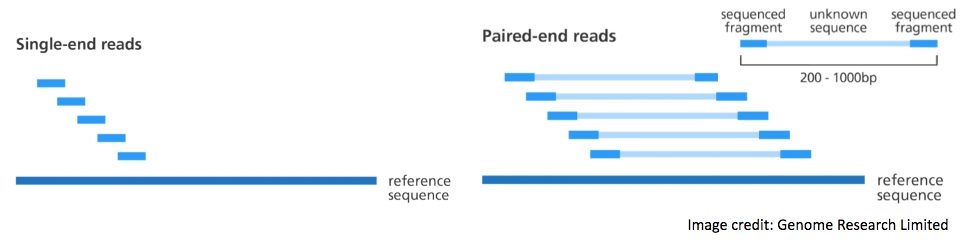
\includegraphics{images/alignment.png}
\caption{NGS Read Alignment}
\end{figure}

    \hypertarget{why-align}{%
\subsubsection{Why align?}\label{why-align}}

There are typical inferences you can make from an alignment of NGS data
against a reference genome:

\begin{itemize}
\tightlist
\item
  Variation from the reference -- could have functional consequence.
\item
  Transcript abundance: Instead of a microarray, you could use alignment
  to genome to quantify expression: more sensitive
\item
  Ab-initio transcript discovery: you can see a pileup from RNA seq data
  showing evidence for an exon which was previously missed or an exon
  which is being skipped in a transcript.
\end{itemize}

    \begin{figure}
\centering
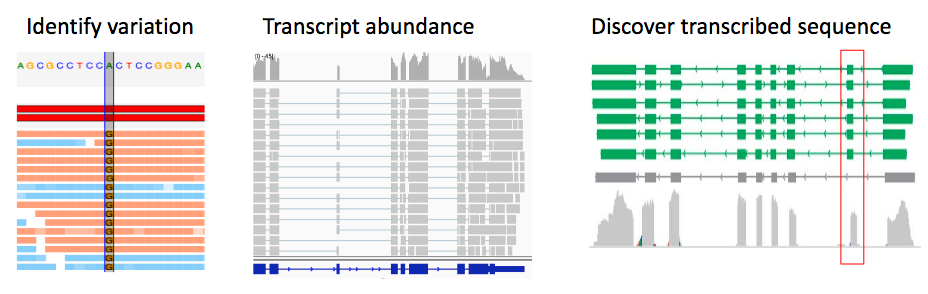
\includegraphics{images/alignment-uses.png}
\caption{Uses of Read Alignment}
\end{figure}

    \hypertarget{learning-outcomes}{%
\subsection{Learning outcomes}\label{learning-outcomes}}

On completion of the tutorial, you can expect to be able to:

\begin{itemize}
\tightlist
\item
  Perform read alignment using standard tools (BWA-MEM)
\item
  Perform the following task and understand their effect on analysis
  results

  \begin{itemize}
  \tightlist
  \item
    Mark Duplicates
  \end{itemize}
\item
  Visualise read alignments using IGV (Integrated Visualisation Tool)
\end{itemize}

If there is time you will learn how to:

\begin{itemize}
\tightlist
\item
  Merge the results from multiple alignments and understand when it is
  appropriate to perform a merge
\end{itemize}

\hypertarget{tutorial-sections}{%
\subsection{Tutorial sections}\label{tutorial-sections}}

This tutorial comprises the following sections:\\
1. \href{alignment.ipynb}{Performing read alignment}\\
2. \href{visualisation.ipynb}{Alignment visualisation}

There is also an additional (optional) section: 3.
\href{workflows.ipynb}{Alignment workflows}

\hypertarget{authors}{%
\subsection{Authors}\label{authors}}

This tutorial was written by
\href{https://github.com/jacquikeane}{Jacqui Keane} based on material
from \href{https://github.com/tk2}{Thomas Keane},
\href{https://github.com/vviyer}{Vivek Iyer} and
\href{https://github.com/vo1}{Victoria Offord}.

\hypertarget{running-the-commands-from-this-tutorial}{%
\subsection{Running the commands from this
tutorial}\label{running-the-commands-from-this-tutorial}}

You can follow this tutorial by typing all the commands you see into a
terminal window. This is similar to the ``Command Prompt'' window on MS
Windows systems, which allows the user to type DOS commands to manage
files.

To get started, open a new terminal on your computer and type the
command below:

    \begin{tcolorbox}[breakable, size=fbox, boxrule=1pt, pad at break*=1mm,colback=cellbackground, colframe=cellborder]
\prompt{In}{incolor}{ }{\boxspacing}
\begin{Verbatim}[commandchars=\\\{\}]
\PY{n+nb}{cd} /home/manager/course\PYZus{}data/read\PYZus{}alignment
\end{Verbatim}
\end{tcolorbox}

    Now you can follow the instructions in the tutorial from here.

\hypertarget{lets-get-started}{%
\subsection{Let's get started!}\label{lets-get-started}}

This tutorial assumes that you have samtools, bwa, Picard tools and IGV
installed on your computer. These are already installed on the VM you
are using. To check that these are installed, you can run the following
commands:

    \begin{tcolorbox}[breakable, size=fbox, boxrule=1pt, pad at break*=1mm,colback=cellbackground, colframe=cellborder]
\prompt{In}{incolor}{ }{\boxspacing}
\begin{Verbatim}[commandchars=\\\{\}]
samtools \PYZhy{}\PYZhy{}help
\end{Verbatim}
\end{tcolorbox}

    \begin{tcolorbox}[breakable, size=fbox, boxrule=1pt, pad at break*=1mm,colback=cellbackground, colframe=cellborder]
\prompt{In}{incolor}{ }{\boxspacing}
\begin{Verbatim}[commandchars=\\\{\}]
bwa
\end{Verbatim}
\end{tcolorbox}

    \begin{tcolorbox}[breakable, size=fbox, boxrule=1pt, pad at break*=1mm,colback=cellbackground, colframe=cellborder]
\prompt{In}{incolor}{ }{\boxspacing}
\begin{Verbatim}[commandchars=\\\{\}]
picard \PYZhy{}h
\end{Verbatim}
\end{tcolorbox}

    \begin{tcolorbox}[breakable, size=fbox, boxrule=1pt, pad at break*=1mm,colback=cellbackground, colframe=cellborder]
\prompt{In}{incolor}{ }{\boxspacing}
\begin{Verbatim}[commandchars=\\\{\}]
igv
\end{Verbatim}
\end{tcolorbox}

    This should return the help message for samtools, bwa and Picard tools
respectively. The final command should launch the genome viewer IGV. You
can close the IGV software, we will use it later in this tutorial to
visualise alignments.

To get started with the tutorial, head to the first section:
\href{alignment.ipynb}{Performing read alignment}


    % Add a bibliography block to the postdoc



\newpage





    \hypertarget{performing-read-alignment}{%
\section{Performing Read Alignment}\label{performing-read-alignment}}

Here we will use the BWA aligner to align a smll set of Illumina
sequencing data to the \textit{Mus Musculus} reference genome. We will
align genomic sequence (from Whole-Genome Sequencing) from a mouse
embryo which has been mutagenised while the one-cell stage using
CRISPR-Cas9 and a gRNA targeting an exon of the Tyr gene. The successful
mutation of the gene will delete one or both alleles. A bi-allelic null
Tyr mouse will be albino, but otherwise healthy.

First, check you are in the correct directory.

    \begin{tcolorbox}[breakable, size=fbox, boxrule=1pt, pad at break*=1mm,colback=cellbackground, colframe=cellborder]
\prompt{In}{incolor}{ }{\boxspacing}
\begin{Verbatim}[commandchars=\\\{\}]
\PY{n+nb}{pwd}
\end{Verbatim}
\end{tcolorbox}

    It should display something like:

\texttt{/home/manager/course\_data/read\_alignment}

    \hypertarget{viewing-the-reference-genome}{%
\subsection{Viewing the reference
genome}\label{viewing-the-reference-genome}}

Go to the \texttt{ref} directory that contains the fasta files of the
reference genomes:

    \begin{tcolorbox}[breakable, size=fbox, boxrule=1pt, pad at break*=1mm,colback=cellbackground, colframe=cellborder]
\prompt{In}{incolor}{ }{\boxspacing}
\begin{Verbatim}[commandchars=\\\{\}]
\PY{n+nb}{cd} \PYZti{}/course\PYZus{}data/read\PYZus{}alignment/data/ref
\end{Verbatim}
\end{tcolorbox}

    Fasta files (.fa) are used to store raw sequencing information before
aligning data. A single chromosome from the mouse genome is contained in
the file GRCm38.68.dna.toplevel.chr7.fa.gz

View the file with zless (we use zless instead of less because the file
is compressed):

    \begin{tcolorbox}[breakable, size=fbox, boxrule=1pt, pad at break*=1mm,colback=cellbackground, colframe=cellborder]
\prompt{In}{incolor}{ }{\boxspacing}
\begin{Verbatim}[commandchars=\\\{\}]
zless GRCm38.68.dna.toplevel.chr7.fa.gz
\end{Verbatim}
\end{tcolorbox}

    \textbf{Q1: What is the length of chromosome 7 of the mouse genome?
(Hint: Look at the fasta header for chromosome 7)}

    \begin{tcolorbox}[breakable, size=fbox, boxrule=1pt, pad at break*=1mm,colback=cellbackground, colframe=cellborder]
\prompt{In}{incolor}{ }{\boxspacing}
\begin{Verbatim}[commandchars=\\\{\}]

\end{Verbatim}
\end{tcolorbox}

    Similar to a BAM file, to allow fast retrieval of data, an index file is
often required. You should check for the presencen of fasta indexes for
the genome in the `ref' directory:

\texttt{GRCm38.68.dna.toplevel.chr7.fa.gz.amb\ ...\ GRCm38.68.dna.toplevel.chr7.fa.gz.sa}

These are created by BWA: suffixtrees, bwt transform etc etc.

If these index files don't exist, then you can run the indexing with the
command

\texttt{bwa\ index\ GRCm38.68.dna.toplevel.chr7.fa.gz}

Beware -- this indexing process can take 3-5 minutes so please only run
it if the index files do not exist!

    \hypertarget{align-the-data-with-bwa}{%
\subsection{Align the data with bwa}\label{align-the-data-with-bwa}}

Go to the
\texttt{\textasciitilde{}/course\_data/read\_alignment/data/Exercise1/fastq/}
directory - you can use this command:

    \begin{tcolorbox}[breakable, size=fbox, boxrule=1pt, pad at break*=1mm,colback=cellbackground, colframe=cellborder]
\prompt{In}{incolor}{ }{\boxspacing}
\begin{Verbatim}[commandchars=\\\{\}]
\PY{n+nb}{cd} ../Exercise1/fastq
\end{Verbatim}
\end{tcolorbox}

    Use the \texttt{bwa\ mem} command to align the fastq files to the mouse
reference genome. By default bwa outputs SAM format directly to the
standard output (in this case your terminal window), therefore you will
have to redirect the result into a SAM file.

    \begin{tcolorbox}[breakable, size=fbox, boxrule=1pt, pad at break*=1mm,colback=cellbackground, colframe=cellborder]
\prompt{In}{incolor}{ }{\boxspacing}
\begin{Verbatim}[commandchars=\\\{\}]
bwa mem ../../ref/GRCm38.68.dna.toplevel.chr7.fa.gz md5638a\PYZus{}7\PYZus{}87000000\PYZus{}R1.fastq.gz md5638a\PYZus{}7\PYZus{}87000000\PYZus{}R2.fastq.gz \PYZgt{} md5638.sam
\end{Verbatim}
\end{tcolorbox}

    This may take a few minutes, please be patient.

    \hypertarget{convert-a-sam-file-to-a-bam-file}{%
\subsection{Convert a SAM file to a BAM
file}\label{convert-a-sam-file-to-a-bam-file}}

Now use samtools to convert the SAM file \texttt{md5638.sam} created in
the previous step into a BAM file called \texttt{md5638.bam}.

    \begin{tcolorbox}[breakable, size=fbox, boxrule=1pt, pad at break*=1mm,colback=cellbackground, colframe=cellborder]
\prompt{In}{incolor}{ }{\boxspacing}
\begin{Verbatim}[commandchars=\\\{\}]
samtools view \PYZhy{}O BAM \PYZhy{}o md5638.bam md5638.sam
\end{Verbatim}
\end{tcolorbox}

    \textbf{Q2: How much space is saved by using a BAM file instead of a SAM
file?}

    \begin{tcolorbox}[breakable, size=fbox, boxrule=1pt, pad at break*=1mm,colback=cellbackground, colframe=cellborder]
\prompt{In}{incolor}{ }{\boxspacing}
\begin{Verbatim}[commandchars=\\\{\}]

\end{Verbatim}
\end{tcolorbox}

    \hypertarget{sort-and-index-the-bam-file}{%
\subsection{Sort and index the BAM
file}\label{sort-and-index-the-bam-file}}

The BAM files produced by BWA are sorted by read name (same order as the
original fastq files). However, most viewing and variant calling
software require the BAM files to be sorted by reference coordinate
position and indexed for rapid retrieval. Therefore, use `samtools sort'
to produce a new BAM file called \texttt{md5638.sorted.bam} that is
sorted by position.

    \begin{tcolorbox}[breakable, size=fbox, boxrule=1pt, pad at break*=1mm,colback=cellbackground, colframe=cellborder]
\prompt{In}{incolor}{ }{\boxspacing}
\begin{Verbatim}[commandchars=\\\{\}]
samtools sort \PYZhy{}T temp \PYZhy{}O bam \PYZhy{}o md5638.sorted.bam md5638.bam
\end{Verbatim}
\end{tcolorbox}

    Finally index the sorted BAM file using `samtools index' command.

\textbf{Note:} indexing a BAM file is also a good way to check that the
BAM file has not been truncated (e.g.~your disk becomes full when
writing the BAM file). At the end of every BAM file, a special end of
file (EOF) marker is written. The Samtools index command will first
check for this and produce an error message if it is not found.

    \begin{tcolorbox}[breakable, size=fbox, boxrule=1pt, pad at break*=1mm,colback=cellbackground, colframe=cellborder]
\prompt{In}{incolor}{ }{\boxspacing}
\begin{Verbatim}[commandchars=\\\{\}]
samtools index md5638.sorted.bam
\end{Verbatim}
\end{tcolorbox}

    \hypertarget{unix-pipes-to-combine-the-commands-together}{%
\subsection{Unix pipes to combine the commands
together}\label{unix-pipes-to-combine-the-commands-together}}

To produce the sorted BAM file above we had to carry out several
separate commands and produce intermediate files. The Unix pipe command
allows you to feed the output of one command into the next command.

You can combine all of these commands together using unix pipes, and do
all of this data processing together and avoid writing intermediate
files. To do this type:

    \begin{tcolorbox}[breakable, size=fbox, boxrule=1pt, pad at break*=1mm,colback=cellbackground, colframe=cellborder]
\prompt{In}{incolor}{ }{\boxspacing}
\begin{Verbatim}[commandchars=\\\{\}]
bwa mem ../../ref/GRCm38.68.dna.toplevel.chr7.fa.gz md5638a\PYZus{}7\PYZus{}87000000\PYZus{}R1.fastq.gz md5638a\PYZus{}7\PYZus{}87000000\PYZus{}R2.fastq.gz \PY{p}{|} samtools view \PYZhy{}O BAM \PYZhy{} \PY{p}{|} samtools sort \PYZhy{}T temp \PYZhy{}O bam \PYZhy{}o md5638\PYZus{}2.sorted.bam \PYZhy{}
\end{Verbatim}
\end{tcolorbox}

    Now index the BAM file:

    \begin{tcolorbox}[breakable, size=fbox, boxrule=1pt, pad at break*=1mm,colback=cellbackground, colframe=cellborder]
\prompt{In}{incolor}{ }{\boxspacing}
\begin{Verbatim}[commandchars=\\\{\}]
samtools index md5638\PYZus{}2.sorted.bam
\end{Verbatim}
\end{tcolorbox}

    \textbf{Note: When the symbol \texttt{-} is used above, Unix will
automatically replace \texttt{-} with the output produced by the
preceeding command (i.e.~the command before the \texttt{\textbar{}}
symbol).}

    \hypertarget{mark-pcr-duplicates}{%
\subsection{Mark PCR Duplicates}\label{mark-pcr-duplicates}}

We will use a program called `MarkDuplicates' that is part of Picard
tools (http://picard.sourceforge.net) to remove PCR duplicates that may
have been introduced during the library construction stage. To find the
options for `MarkDuplicates' -- type:

    \begin{tcolorbox}[breakable, size=fbox, boxrule=1pt, pad at break*=1mm,colback=cellbackground, colframe=cellborder]
\prompt{In}{incolor}{ }{\boxspacing}
\begin{Verbatim}[commandchars=\\\{\}]
picard MarkDuplicates
\end{Verbatim}
\end{tcolorbox}

    Now run MarkDuplicates using the `I=' option to specify the input BAM
file and the `O=' option to specify the output file
(e.g.~md5638.markdup.bam). You will also need to specify the duplication
metrics output file using `M=' (e.g.~md5638.markdup.metrics).

    \begin{tcolorbox}[breakable, size=fbox, boxrule=1pt, pad at break*=1mm,colback=cellbackground, colframe=cellborder]
\prompt{In}{incolor}{ }{\boxspacing}
\begin{Verbatim}[commandchars=\\\{\}]
picard MarkDuplicates \PY{n+nv}{I}\PY{o}{=}md5638.sorted.bam \PY{n+nv}{O}\PY{o}{=}md5638.markdup.bam \PY{n+nv}{M}\PY{o}{=}md5638.metrics.txt
\end{Verbatim}
\end{tcolorbox}

    \textbf{Q3: From looking at the output metrics file - how many reads
were marked as duplicates? What was the percent duplication?}

    \begin{tcolorbox}[breakable, size=fbox, boxrule=1pt, pad at break*=1mm,colback=cellbackground, colframe=cellborder]
\prompt{In}{incolor}{ }{\boxspacing}
\begin{Verbatim}[commandchars=\\\{\}]

\end{Verbatim}
\end{tcolorbox}

    Don't forget to generate an index for the new bam file using samtools.

    \begin{tcolorbox}[breakable, size=fbox, boxrule=1pt, pad at break*=1mm,colback=cellbackground, colframe=cellborder]
\prompt{In}{incolor}{ }{\boxspacing}
\begin{Verbatim}[commandchars=\\\{\}]
samtools index md5638.markdup.bam
\end{Verbatim}
\end{tcolorbox}

    \hypertarget{generate-qc-stats}{%
\subsection{Generate QC Stats}\label{generate-qc-stats}}

Use samtools to collect some statistics and generate QC plots from the
alignment in the BAM file from the previous step. Make sure you save the
output of the stats command to a file
(e.g.~\texttt{md5638.markdup.stats}).

    \begin{tcolorbox}[breakable, size=fbox, boxrule=1pt, pad at break*=1mm,colback=cellbackground, colframe=cellborder]
\prompt{In}{incolor}{ }{\boxspacing}
\begin{Verbatim}[commandchars=\\\{\}]
samtools stats md5638.markdup.bam \PYZgt{} md5638.markdup.stats
\end{Verbatim}
\end{tcolorbox}

    \begin{tcolorbox}[breakable, size=fbox, boxrule=1pt, pad at break*=1mm,colback=cellbackground, colframe=cellborder]
\prompt{In}{incolor}{ }{\boxspacing}
\begin{Verbatim}[commandchars=\\\{\}]
plot\PYZhy{}bamstats \PYZhy{}p md5638\PYZus{}plot/ md5638.markdup.stats
\end{Verbatim}
\end{tcolorbox}

    \hypertarget{exercises}{%
\subsection{Exercises}\label{exercises}}

Now look at the output and answer the following questions:

\textbf{Q4: What is the total number of reads?}

\textbf{Q5: What proportion of the reads were mapped?}

\textbf{Q6: How many reads were paired correctly/properly?}

\textbf{Q7: How many read pairs mapped to a different chromosome?}

\textbf{Q8: What is the insert size mean and standard deviation?}

In your web browser open the file called md5638\_plot.html to view the
QC information and anser the following questions:

\textbf{Q9: How many reads have zero mapping quality?}

\textbf{Q10: Which of the first fragments or second fragments are higher
base quality on average?}

    Congratulations you have succesfully aligned some NGS data to a
reference genome! Now continue to the next section of the tutorial:
\href{visualisation.ipynb}{Alignment visualisation}.


    % Add a bibliography block to the postdoc



\newpage





    \hypertarget{alignment-visualisation}{%
\section{Alignment Visualisation}\label{alignment-visualisation}}

You have now made it to the interesting part!

Integrative Genome Viewer (IGV) \url{http://www.broadinstitute.org/igv/}
allows you to visualise genomic datasets and is a very useful tool for
looking at the alignment of reads onto a reference genome from BAM
files.

Start IGV by typing:

    \begin{tcolorbox}[breakable, size=fbox, boxrule=1pt, pad at break*=1mm,colback=cellbackground, colframe=cellborder]
\prompt{In}{incolor}{ }{\boxspacing}
\begin{Verbatim}[commandchars=\\\{\}]
igv \PY{p}{\PYZam{}}
\end{Verbatim}
\end{tcolorbox}

    \hypertarget{igv-main-window}{%
\subsection{IGV main window}\label{igv-main-window}}

When you start IGV, it will open a main window. At the top of this
window you have a toolbar and genome ruler for navigation. The largest
area in the main window is the data viewer where your alignments,
annotations and other data will be displayed. To do this, IGV uses
horizontal rows called tracks. Finally, at the bottom, there is a
sequence viewer which contains the base level information for your
reference genome.

    \begin{figure}
\centering
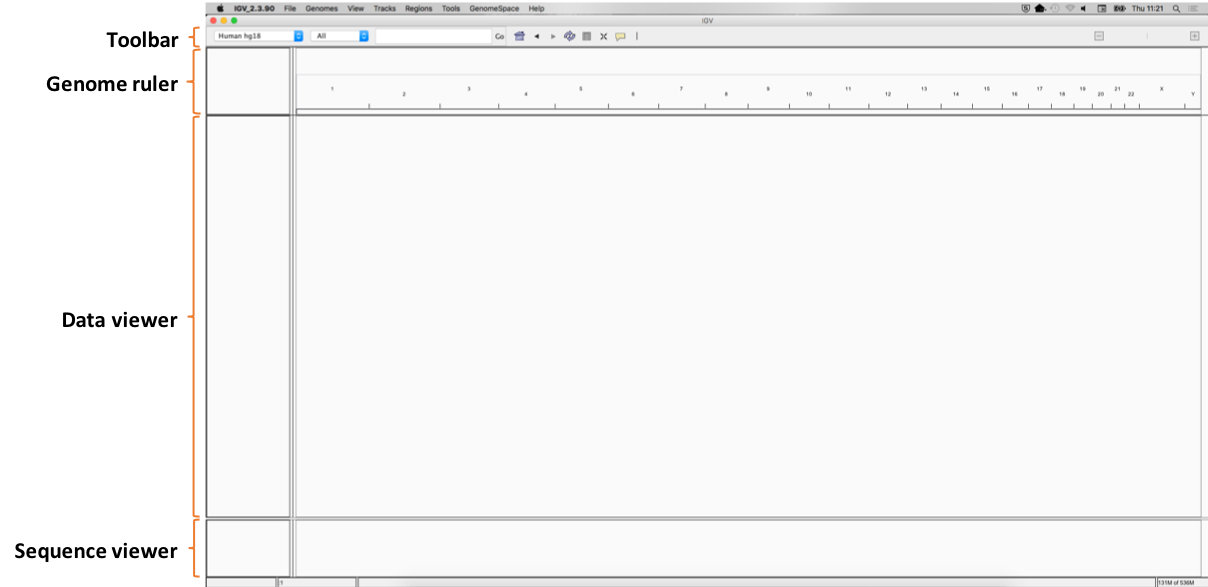
\includegraphics{images/igv-main-window.png}
\caption{IGV - main window}
\end{figure}

    \hypertarget{load-the-reference-genome}{%
\subsection{Load the reference genome}\label{load-the-reference-genome}}

IGV provides several genomes which can be selected with the ``Genome
drop-down box'' on the toolbar.

\textbf{Go to ' \textit{Genomes -\textgreater{} Load Genome From
Server\ldots{}} ' and select ``Mouse mm10''. This is a synonym for
GRCm38, which is the current mouse assembly (reference genome)}

    \begin{figure}
\centering
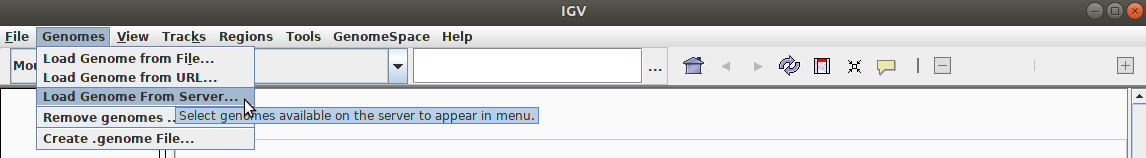
\includegraphics{images/load-mouse-ref.png}
\caption{IGV - loading the mouse genome}
\end{figure}

    \begin{figure}
\centering
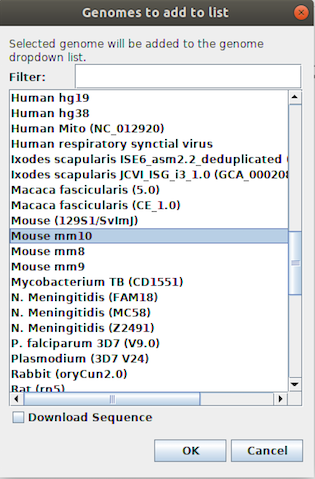
\includegraphics{images/mouse-ref-dialog.png}
\caption{IGV - list of available genomes}
\end{figure}

    \hypertarget{igv-toolbar-and-genome-ruler}{%
\subsubsection{IGV toolbar and genome
ruler}\label{igv-toolbar-and-genome-ruler}}

Once the genome has loaded, the chromosomes will be shown on the
\textbf{genome ruler} with their names/numbers above. When a region is
selected, a red box will appear. This represents the visible region of
the genome.

Above the genome ruler is the \textbf{toolbar} which has a variety
controls for navigating the genome:

\begin{itemize}
\tightlist
\item
  \textbf{Genome drop-down} - load a genome
\item
  \textbf{Chromosome drop-down} - zoom to a chromosome
\item
  \textbf{Search} - zoom to a chromosome, locus or gene
\end{itemize}

There are several other buttons which can be used to control the visible
portion of the genome.

\begin{itemize}
\tightlist
\item
  \textbf{Whole genome} - zoom back out to whole genome view
\item
  \textbf{Previous/next view} - move backward/forward through views
  (like the back/forward buttons in a web browser)
\item
  \textbf{Refresh} - refresh the display
\item
  \textbf{Zoom} - zooms in (+) / out (-) on a chromosome
\end{itemize}

    \begin{figure}
\centering
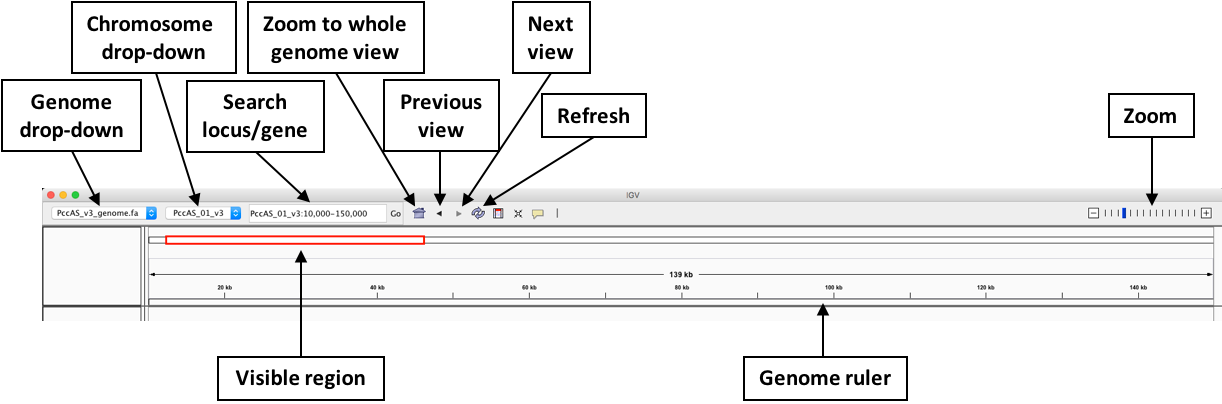
\includegraphics{images/igv-toolbar.png}
\caption{IGV - toolbar and genome ruler}
\end{figure}

    \hypertarget{sequence-viewer}{%
\subsubsection{Sequence viewer}\label{sequence-viewer}}

The \textbf{sequence viewer} shows the genome at the single nucleotide
level. You won't be able to see the sequence until you are zomed in.
Let's try it, select the zooom in (+) option in the top right of the
screeen. As you start to zoom in (+), you will see that each nucleotide
is represented by a coloured bar (red=T, yellow=G, blue=C and green=A).
This makes it easier to spot repetitive regions in the genome. Carry on
zooming in (+) and you will see the individual nucleotides.

    \begin{figure}
\centering
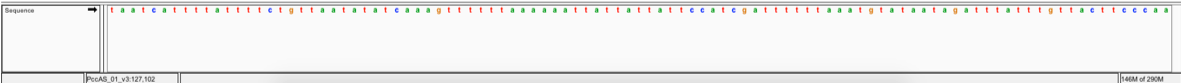
\includegraphics{images/igv-sequence-viewer.png}
\caption{IGV - sequence viewer}
\end{figure}

    \hypertarget{navigation-in-igv}{%
\subsection{Navigation in IGV}\label{navigation-in-igv}}

There are several views in IGV

\begin{itemize}
\tightlist
\item
  Genome view
\item
  Chromosome view
\item
  Region view
\end{itemize}

There are several ways to to zoom in and out to these views to look at
specific regions or base level information.

    \hypertarget{whole-genome-view}{%
\subsubsection{Whole genome view}\label{whole-genome-view}}

To get a view of the entire genome select the zoom to whole genome icon
(house icon) found in the toolbar at the top of the IGV window.

    \begin{figure}
\centering
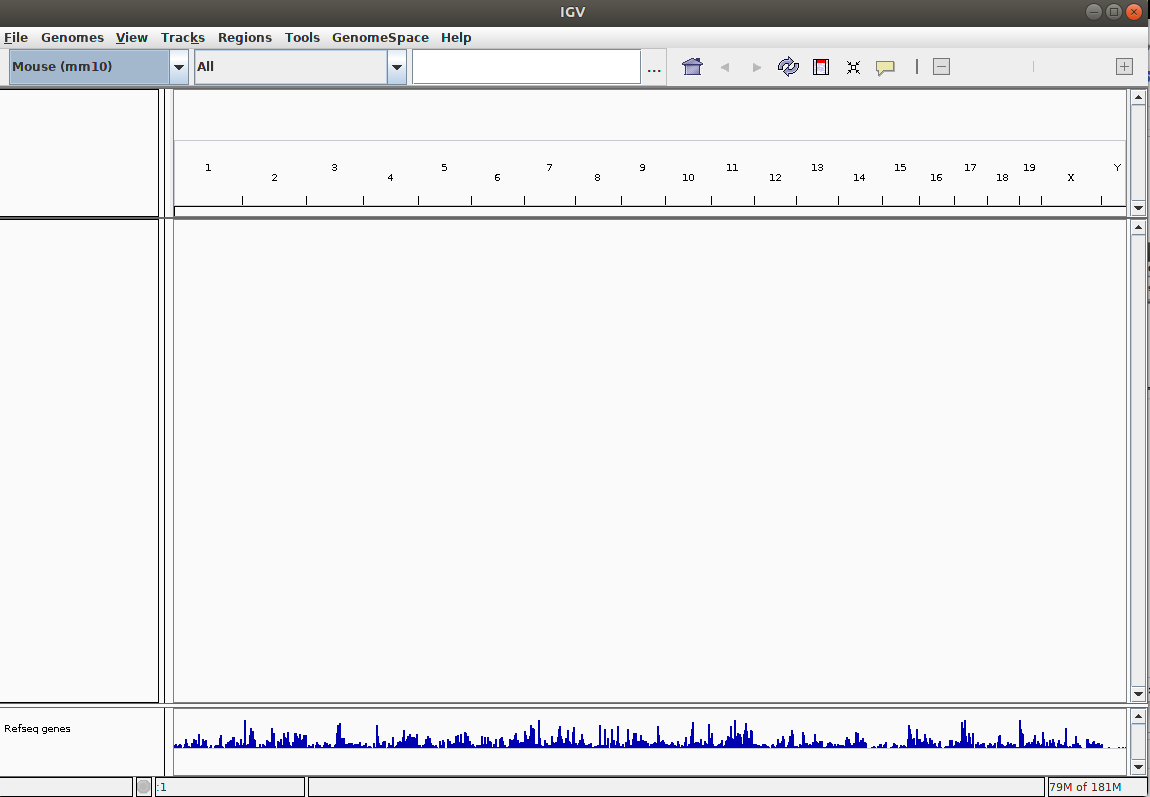
\includegraphics{images/whole-genome-view.png}
\caption{IGV - whole genome view}
\end{figure}

    \hypertarget{chromosome-view}{%
\subsubsection{Chromosome view}\label{chromosome-view}}

To get a view of a specific chromosome select the chromosome from the
chromosome drop down list in the toolbar of the IGV window.

    \begin{figure}
\centering
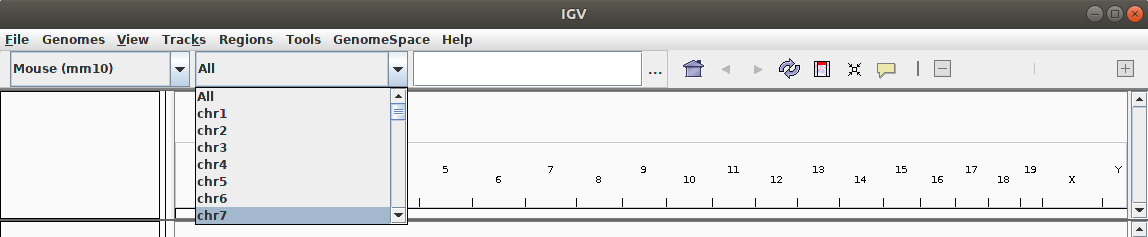
\includegraphics{images/chromosome-view.png}
\caption{IGV - chromosome view}
\end{figure}

    \hypertarget{region-view}{%
\subsubsection{Region view}\label{region-view}}

\hypertarget{jump-to-region}{%
\paragraph{Jump to region}\label{jump-to-region}}

If you know the co-ordinates of the region you want to view, you can
enter them into the ``\textit{Search}'' and click ``\textit{Go}''. The
format is chromosome:start-stop. For example, to view from 100,000 to
100,100 on chr7, you would enter chr7:100,000-100,100 in the search box.
We will practice this later in an exercise.

    \hypertarget{select-region}{%
\paragraph{Select region}\label{select-region}}

If you don't know the specific co-ordinates of the region you want to
look at, you can click and drag to select a region on the genome
toolbar.

    \begin{figure}
\centering
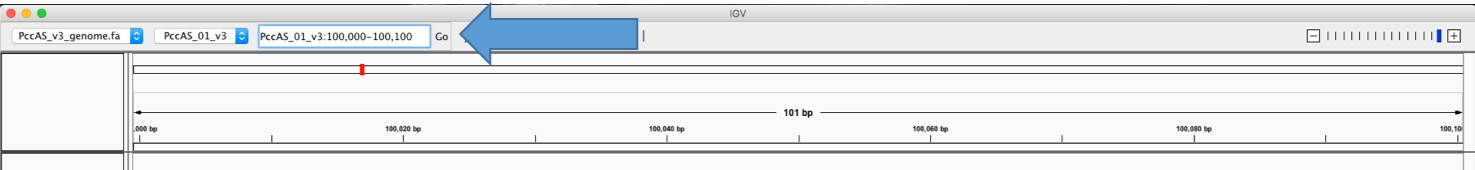
\includegraphics{images/igv-search-region.png}
\caption{IGV - search region}
\end{figure}

    \textit{Note: the visible region of the chromosome is indicated by the red
box on the genome ruler.}

    \hypertarget{zooming-in-and-out}{%
\subsubsection{Zooming in and out}\label{zooming-in-and-out}}

You can zoom in and out from each view by using the ``+'' and ``-''
buttons on the zoom control at the right-hand side of the toolbar. This
will also work with the ``+'' and ``-'' keys on your keyboard.

    \begin{figure}
\centering
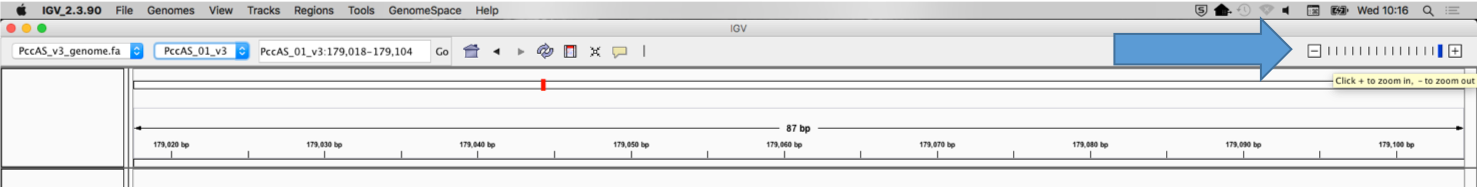
\includegraphics{images/igv-zoom-in-out.png}
\caption{IGV - zoom in/out}
\end{figure}

    \hypertarget{load-the-alignment}{%
\subsection{Load the alignment}\label{load-the-alignment}}

IGV can be used to visualise many different types of data, including
read alignments. Each time you load an alignment file it will be added
to the \textbf{data viewer} as a new major \textbf{track}.

\textbf{Go to ' \textit{File -\textgreater{} Load from File\ldots{}} `.
Select the ``md5638.markdup.bam'' BAM file that you created in the
previous section and click' \textit{Open} '.}

    \begin{figure}
\centering
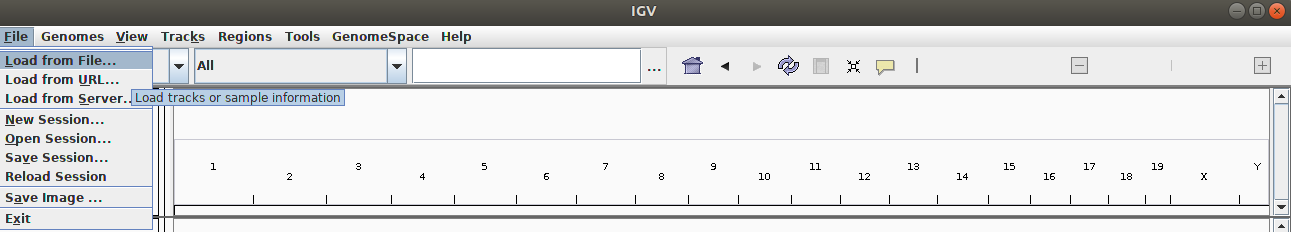
\includegraphics{images/igv-load-alignment-1.png}
\caption{IGV - loading alignment from file}
\end{figure}

    \begin{figure}
\centering
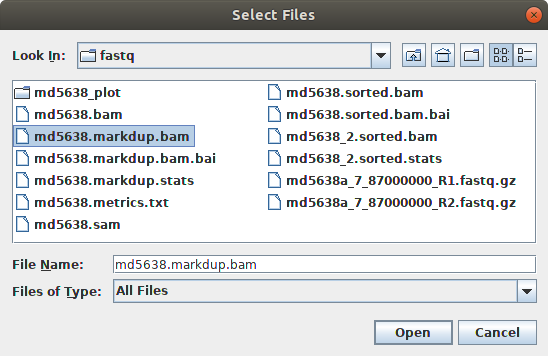
\includegraphics{images/igv-load-alignment-2.png}
\caption{IGV - loading alignment from file}
\end{figure}

    \textbf{Note:} BAM files and their corresponding index files must be in
the same directory for IGV to load them properly.

For each read alignment, a major track will appear containing two minor
tracks for that sample:

\begin{itemize}
\tightlist
\item
  coverage information
\item
  read alignments
\end{itemize}

For the total number of visible tracks, see the bottom left of main
window.

At the genome level view, there will be no coverage plot or read
alignments visible. At the chromosome level view, there are two messages
displayed: Zoom in to see coverage/alignments. Finally, once you have
zoomed in (+) you will see a density plot in the coverage track and your
read alignments.

    \begin{figure}
\centering
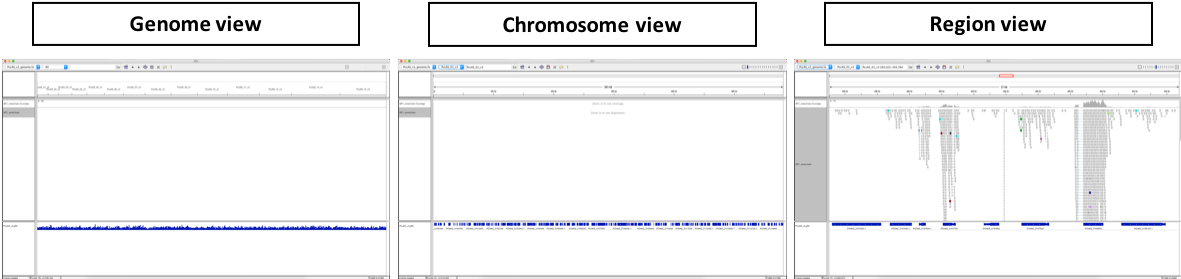
\includegraphics{images/igv-alignment-views.png}
\caption{IGV - alignment views}
\end{figure}

    \hypertarget{visualising-alignments}{%
\subsection{Visualising alignments}\label{visualising-alignments}}

\hypertarget{coverage-information}{%
\subsubsection{Coverage information}\label{coverage-information}}

When zoomed in to view a region, you can get alignment information for
each position in the genome by hovering over the coverage track. This
will open a yellow box which tells you the total number of reads mapped
at that position, a breakdown of the mapped nucleotide frequencies and
the number of reads mapping in a forward/reverse orientation. In the
example shown below, 95 reads mapped, 50 forward and 45 reverse, all of
which called A at position 202,768 on chromosome PccAS\_05\_v3. This is
just an example for illustrative purposes, please do not try to look at
this position in IGV here.

    \begin{figure}
\centering
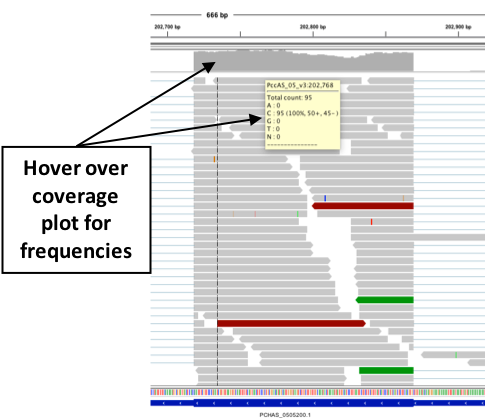
\includegraphics{images/igv-coverage-stats.png}
\caption{IGV - coverage information}
\end{figure}

    \hypertarget{viewing-individual-read-alignment-information}{%
\subsubsection{Viewing individual read alignment
information}\label{viewing-individual-read-alignment-information}}

Read are represented by grey or transparent/white bars which are stacked
together where they align to the reference genome. Reads are pointed to
indicate the orientation in which they mapped i.e.~on the forward or
reverse strand. Hovering over an individual read will display
information about its alignment.

(images/igv-read-information.png ``IGV - read information'')

Mismatches occur where the nucleotide in the aligned read is not the
same as the nucleotide in that position on the reference genome. A
mismatch is indicated by a coloured bar at the relevant position on the
read. The colour of the bar represents the mismatched base in the read
(red=T, yellow=G, blue=C and green=A).

    \begin{figure}
\centering

\includegraphics{images/igv-mismatch.png}
\caption{IGV - mismatch}
\end{figure}

    \hypertarget{igv-configuration}{%
\subsection{IGV configuration}\label{igv-configuration}}

Follow the instructions that follow to set up your IGV view:

\textbf{Select the little yellow ``speech bubble'' icon in the toolbar
and set the option to ``Show Details on Click'' (or you will go mad, I
promise!).}

    \begin{figure}
\centering
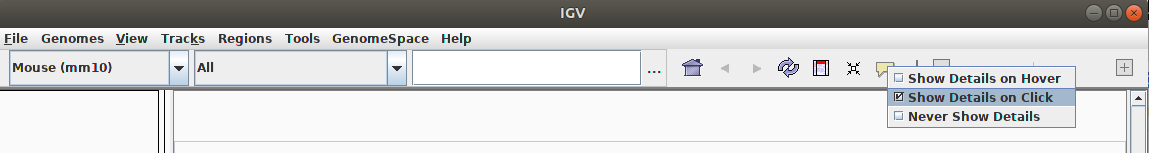
\includegraphics{images/igv-set-popup-on-click.png}
\caption{IGV Set popups on click only}
\end{figure}

    \textbf{Zoom in so you can see sequence reads and go to region
chr7:87480000-87485000 using the navigation bar at the top.}

    \begin{figure}
\centering
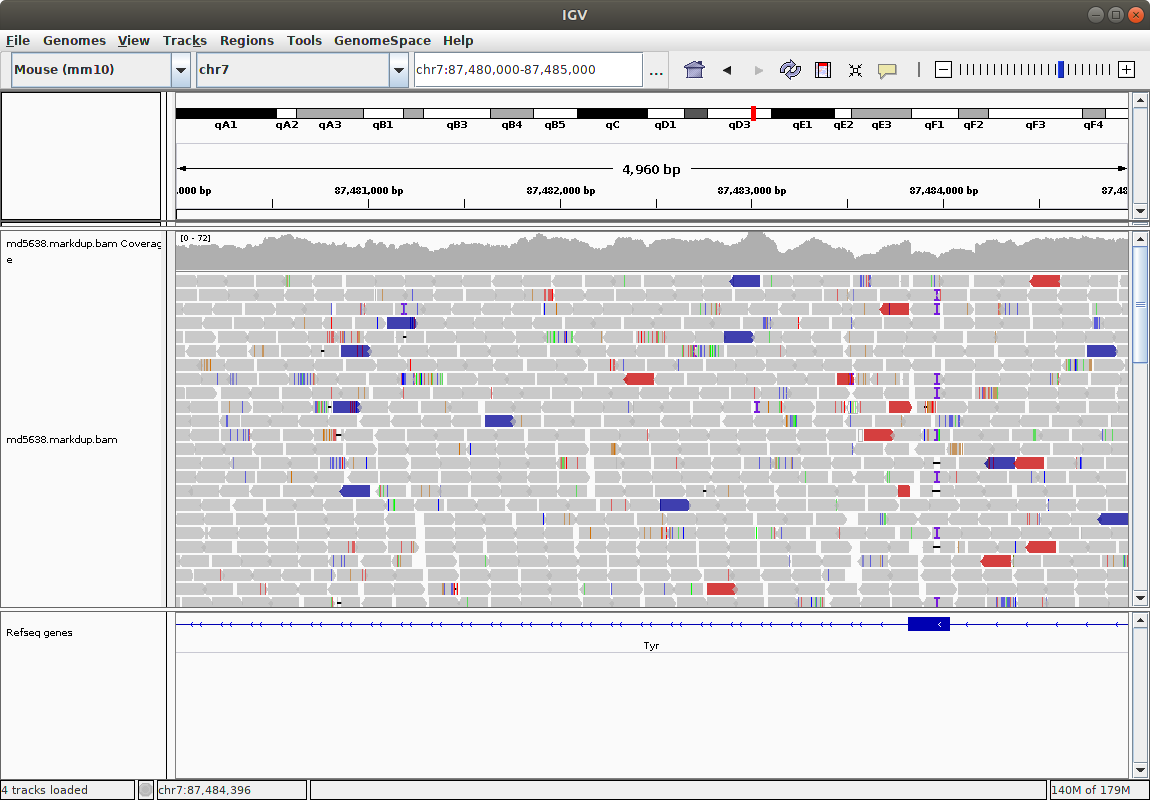
\includegraphics{images/igv-chr7-zoomed-view.png}
\caption{IGV - View of region of chromosome 7}
\end{figure}

    \textbf{Control-click or right-click in the data view window. Choose
sort alignments by insert size, then choose colour alignments by insert
size and finally choose ``View as pairs''.}

\textbf{Go to ' \textit{View -\textgreater{} Preferences\ldots{}} ' select
the ' \textit{Alignments} ' tab and ensure the ``Show soft-clipped bases''
option is ticked. This colour highlighting emphasises soft-clips on the
read itself.}

    \begin{figure}
\centering
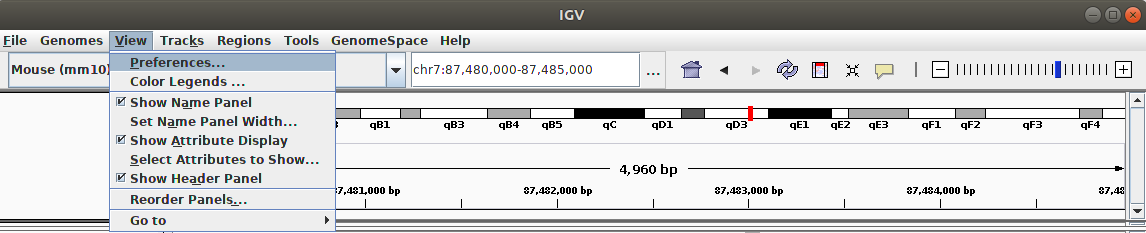
\includegraphics{images/igv-configure-soft-clip-1.png}
\caption{IGV - Configuring the view}
\end{figure}

    \begin{figure}
\centering
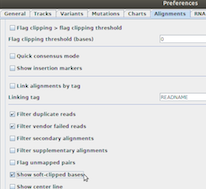
\includegraphics{images/igv-configure-soft-clip-2.png}
\caption{IGV - Configuring the view}
\end{figure}

    Your IGV session should look similar to:

    \begin{figure}
\centering
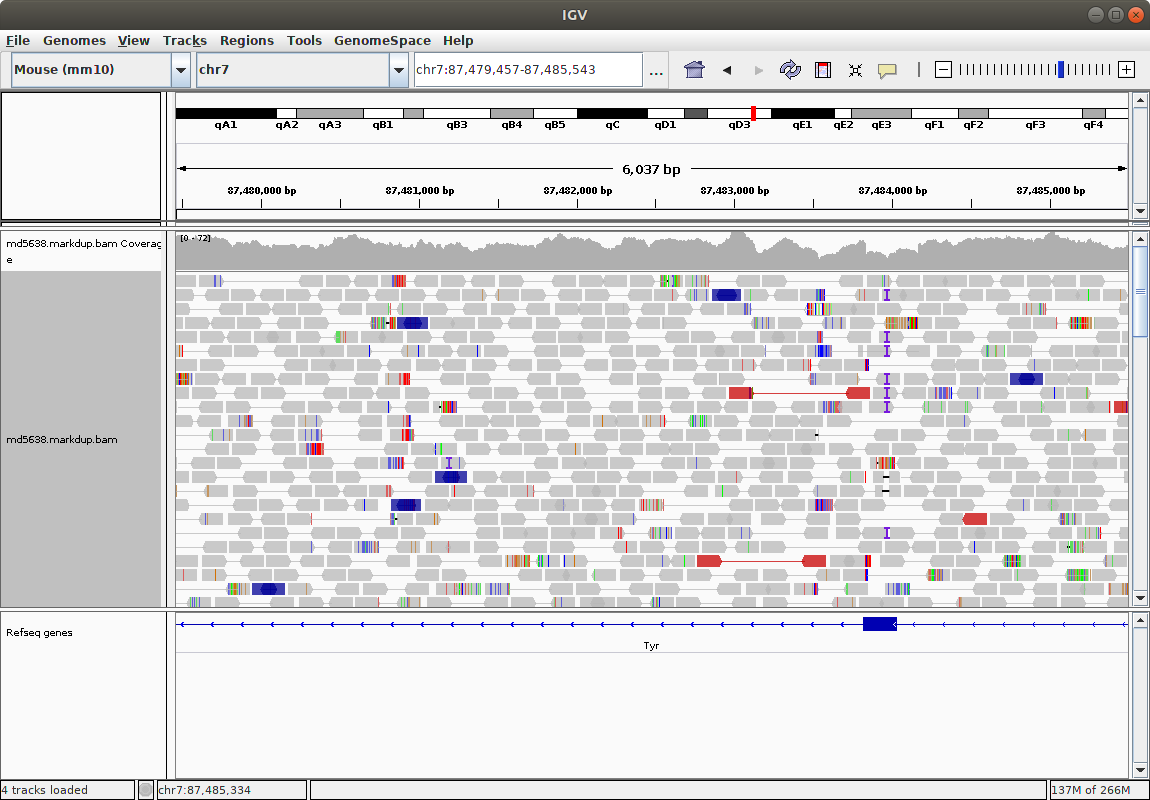
\includegraphics{images/igv-final-view.png}
\caption{IGV}
\end{figure}

    \hypertarget{exercises}{%
\subsection{Exercises}\label{exercises}}

\begin{enumerate}
\def\labelenumi{\arabic{enumi}.}
\item
  Go to chromosome chr7, positions 87,483,625-87,484,330 using the
  navigation bar across the top. Take in the glorious view of a genome
  pileup. Stop and smell the roses! Click on stuff! Scroll around, zoom
  in and out a bit!
\item
  Go back to chromosome 7:87,483,625-87,484,330. What is the (rough)
  coverage across this region? (\textbf{Hint:} Look at the coverage
  track)
\item
  Can you spot the three mutant variants (two small and one larger) in
  this region? State what the evidence is for them?
\end{enumerate}

\textbf{Hints}

\begin{itemize}
\tightlist
\item
  Hint1: Look around 87,483,960 for an insertion. How large is it? How
  many reads does it occur in?
\item
  Hint2: Look around 87,483,960 for a deletion. How large is it? How
  many reads does it occur in?
\item
  Hint3: Zoom out slightly and watch the coverage track between
  87,483,700 - 87,484,200. Once you've spotted the large change look at
  reference sequence the edges of the mutation to hazard a guess as to
  its mechanism.
\end{itemize}

\begin{enumerate}
\def\labelenumi{\arabic{enumi}.}
\setcounter{enumi}{3}
\tightlist
\item
  Can you venture a guess as to what happened here? Why are these
  mutations present?
\end{enumerate}

    \textbf{Congratulations} you have completed the Read Alignment tutorial.
If you have time left then continue to the next (optional) section of
the tutorial: \href{workflows.ipynb}{Alignment workflows}.

    Here is an additional IGV tutorial and refresher:
\url{https://github.com/sanger-pathogens/pathogen-informatics-training/blob/master/Notebooks/IGV/IGV.pdf}.
You can find a copy of this tutorial in your manual. Unfortunately,
there is not enough time to complete this tutorial now but you may find
it useful to look at it after the course.


    % Add a bibliography block to the postdoc



\newpage





    \hypertarget{ngs-workflows}{%
\section{NGS Workflows}\label{ngs-workflows}}

A typical NGS experiment involves more than one sample, potential 10's
or 100's of samples. During the experiment, a sample may be split across
multiple libraries and and a library may be split across multiple
sequencing runs (lanes). For example, you may have to increase the
number of runs for a specific sample to increase the read-depth
(sequencing volume), so you have to prepare multiple libraries.

Therefore you need a coordinated workflow, driven by standard software
to bring it reliably together. Read alignment is just the first part of
that. Once you have a BAM file for each sequencing run you need to merge
them together to produce a BAM file for the library. At this stage it is
important to perform de-duplication on the merged data. The main purpose
of removing duplicates is to mitigate the effects of PCR amplification
bias introduced during library construction. PCR duplicates erroneously
inflate the coverage and, if not removed, can give the illusion of high
confidence when it is not really there which can have an effect on
downstream analysis such as variant calling.

The figure below outlines a typical NGS workflow:

    \begin{figure}
\centering
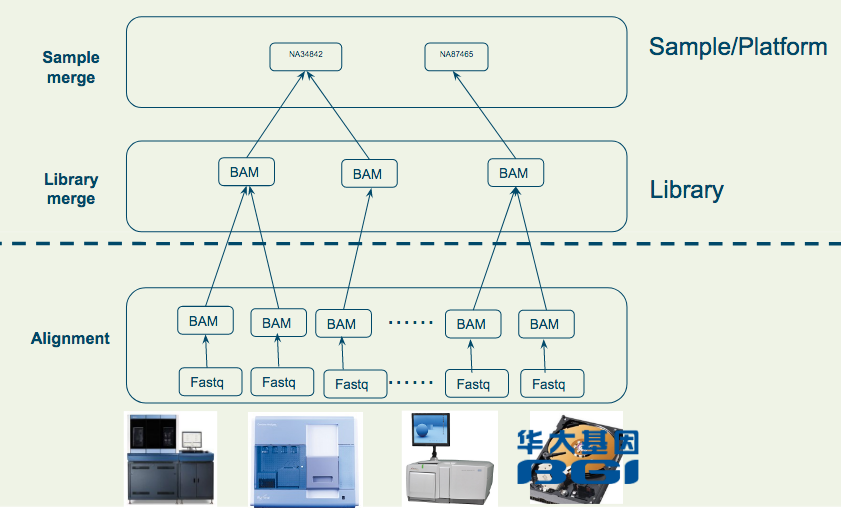
\includegraphics{images/workflow.png}
\caption{Typical NGS Workflow}
\end{figure}

    In this part of the tutotial, we have two lanes of illumina sequencing
data produced from a single library of yeast. We will use the BWA
aligner to align the data to the Saccromyces cerevisiae genome
(ftp://ftp.ensembl.org/pub/current\_fasta/saccharomyces\_cerevisiae/dna/)
and produce a merged BAM file for the library.

To begin go to the following directory:

    \begin{tcolorbox}[breakable, size=fbox, boxrule=1pt, pad at break*=1mm,colback=cellbackground, colframe=cellborder]
\prompt{In}{incolor}{ }{\boxspacing}
\begin{Verbatim}[commandchars=\\\{\}]
\PY{n+nb}{cd} /home/manager/course\PYZus{}data/read\PYZus{}alignment/data/Exercise2/60A\PYZus{}Sc\PYZus{}DBVPG6044/library1
\end{Verbatim}
\end{tcolorbox}

    \hypertarget{index-the-reference}{%
\subsection{Index the reference}\label{index-the-reference}}

    \begin{tcolorbox}[breakable, size=fbox, boxrule=1pt, pad at break*=1mm,colback=cellbackground, colframe=cellborder]
\prompt{In}{incolor}{ }{\boxspacing}
\begin{Verbatim}[commandchars=\\\{\}]
bwa index ../../../../ref/Saccharomyces\PYZus{}cerevisiae.R64\PYZhy{}1\PYZhy{}1.dna.toplevel.fa.gz
\end{Verbatim}
\end{tcolorbox}

    \hypertarget{align-the-first-sequencing-run}{%
\subsection{Align the first sequencing
run}\label{align-the-first-sequencing-run}}

Recall that to align a lane of data to a reference genome we must
perform the following steps:

\begin{itemize}
\tightlist
\item
  Align the data
\item
  Convert from SAM to BAM
\item
  Sort the BAM file
\item
  Index the sorted BAM file
\end{itemize}

\hypertarget{find-the-data}{%
\subsubsection{Find the data}\label{find-the-data}}

Go to the directory that contains the data for the first sequencing run:

    \begin{tcolorbox}[breakable, size=fbox, boxrule=1pt, pad at break*=1mm,colback=cellbackground, colframe=cellborder]
\prompt{In}{incolor}{ }{\boxspacing}
\begin{Verbatim}[commandchars=\\\{\}]
\PY{n+nb}{cd} lane1
\end{Verbatim}
\end{tcolorbox}

    \hypertarget{run-the-alignment}{%
\subsubsection{Run the alignment}\label{run-the-alignment}}

Remember from earlier in the tutorial that the Unix pipe command allows
you to feed the output of one command into the next command. So using
Unix pipes, we can combine all of the alignment steps together into one
command and do all of this data processing together and avoid writing
intermediate files. To do this type the command:

    \begin{tcolorbox}[breakable, size=fbox, boxrule=1pt, pad at break*=1mm,colback=cellbackground, colframe=cellborder]
\prompt{In}{incolor}{ }{\boxspacing}
\begin{Verbatim}[commandchars=\\\{\}]
bwa mem \PYZhy{}M \PYZhy{}R \PY{l+s+s1}{\PYZsq{}@RG\PYZbs{}tID:lane1\PYZbs{}tSM:60A\PYZus{}Sc\PYZus{}DBVPG6044\PYZsq{}} ../../../../ref/Saccharomyces\PYZus{}cerevisiae.R64\PYZhy{}1\PYZhy{}1.dna.toplevel.fa.gz s\PYZus{}7\PYZus{}1.fastq.gz s\PYZus{}7\PYZus{}2.fastq.gz \PY{p}{|} samtools view \PYZhy{}bS \PYZhy{} \PY{p}{|} samtools sort \PYZhy{}T temp \PYZhy{}O bam \PYZhy{}o lane1.sorted.bam \PYZhy{}
\end{Verbatim}
\end{tcolorbox}

    \textbf{Q1: What do the -M and -R options do?}

    \textbf{Q2: What does the -bS option do?}

    Now index the BAM file:

    \begin{tcolorbox}[breakable, size=fbox, boxrule=1pt, pad at break*=1mm,colback=cellbackground, colframe=cellborder]
\prompt{In}{incolor}{ }{\boxspacing}
\begin{Verbatim}[commandchars=\\\{\}]
samtools index lane1.sorted.bam
\end{Verbatim}
\end{tcolorbox}

    \hypertarget{generate-qc-stats}{%
\subsubsection{Generate QC stats}\label{generate-qc-stats}}

Now use samtools to collect some statistics and generate QC plots from
the alignment in the BAM file. Type the commands:

    \begin{tcolorbox}[breakable, size=fbox, boxrule=1pt, pad at break*=1mm,colback=cellbackground, colframe=cellborder]
\prompt{In}{incolor}{ }{\boxspacing}
\begin{Verbatim}[commandchars=\\\{\}]
samtools stats lane1.sorted.bam \PYZgt{} lane1.stats.txt
\end{Verbatim}
\end{tcolorbox}

    \begin{tcolorbox}[breakable, size=fbox, boxrule=1pt, pad at break*=1mm,colback=cellbackground, colframe=cellborder]
\prompt{In}{incolor}{ }{\boxspacing}
\begin{Verbatim}[commandchars=\\\{\}]
plot\PYZhy{}bamstats \PYZhy{}p plot/ lane1.stats.txt
\end{Verbatim}
\end{tcolorbox}

    Now look at the output and answer the following questions:

\textbf{Q3:} What is the total number of reads?

\textbf{Q4:} What proportion of the reads were mapped?

\textbf{Q5:} How many reads were paired correctly/properly?

\textbf{Q6:} How many reads mapped to a different chromosome?

\textbf{Q7:} What is the insert size mean and standard deviation?

In a web browser open the file called plots.html to view the QC
information.

\textbf{Q8:} How many reads have zero mapping quality?

\textbf{Q9:} Which of the first fragments or second fragments are higher
base quality on average?

    \hypertarget{align-the-second-sequencing-run}{%
\subsection{Align the second sequencing
run}\label{align-the-second-sequencing-run}}

There is a second lane of sequencing data in the \texttt{library1}
directory contained in the directory \texttt{lane2}. We want to also
align this sequncing data and produce a BAM file.

Go to the directory that contains the data for the second sequencing
run:

    \begin{tcolorbox}[breakable, size=fbox, boxrule=1pt, pad at break*=1mm,colback=cellbackground, colframe=cellborder]
\prompt{In}{incolor}{ }{\boxspacing}
\begin{Verbatim}[commandchars=\\\{\}]
\PY{n+nb}{cd} ../lane2
\end{Verbatim}
\end{tcolorbox}

    Now align the data in this directory to the yeast reference genome and
produce a sorted BAM file.

\textbf{Note:} This time when you use the \texttt{bwa\ mem} command use
the following header option to specify lane2 as the read group ID:

\texttt{@RG\textbackslash{}tID:lane2\textbackslash{}tSM:60A\_Sc\_DBVPG6044}

    \begin{tcolorbox}[breakable, size=fbox, boxrule=1pt, pad at break*=1mm,colback=cellbackground, colframe=cellborder]
\prompt{In}{incolor}{ }{\boxspacing}
\begin{Verbatim}[commandchars=\\\{\}]

\end{Verbatim}
\end{tcolorbox}

    \textbf{Q10:} What is the size of the BAM file that is produced?

    \hypertarget{merge-the-bam-files}{%
\subsection{Merge the BAM files}\label{merge-the-bam-files}}

Go to the directory that contains the data for the library
\texttt{60A\_Sc\_DBVPG6044/library1} . Use \texttt{ls} to get a listing
of the files and directories contained in this directory.

    \begin{tcolorbox}[breakable, size=fbox, boxrule=1pt, pad at break*=1mm,colback=cellbackground, colframe=cellborder]
\prompt{In}{incolor}{ }{\boxspacing}
\begin{Verbatim}[commandchars=\\\{\}]
\PY{n+nb}{cd} ..
\end{Verbatim}
\end{tcolorbox}

    \begin{tcolorbox}[breakable, size=fbox, boxrule=1pt, pad at break*=1mm,colback=cellbackground, colframe=cellborder]
\prompt{In}{incolor}{ }{\boxspacing}
\begin{Verbatim}[commandchars=\\\{\}]
\PY{n+nb}{pwd}
\end{Verbatim}
\end{tcolorbox}

    \begin{tcolorbox}[breakable, size=fbox, boxrule=1pt, pad at break*=1mm,colback=cellbackground, colframe=cellborder]
\prompt{In}{incolor}{ }{\boxspacing}
\begin{Verbatim}[commandchars=\\\{\}]
ls
\end{Verbatim}
\end{tcolorbox}

    You will notice that there are two directories called \texttt{lane1} and
\texttt{lane2}. There were two sequencing lanes produced from this
sequencing library. In order to mark library PCR duplicates, we need to
merge the two lane BAM files together to produce a single BAM file. We
will use the picard tool called `MergeSamFiles'
(http://picard.sourceforge.net) to merge the lane BAM files.

To find the options for `MergeSamFiles' command, type:

    \begin{tcolorbox}[breakable, size=fbox, boxrule=1pt, pad at break*=1mm,colback=cellbackground, colframe=cellborder]
\prompt{In}{incolor}{ }{\boxspacing}
\begin{Verbatim}[commandchars=\\\{\}]
picard MergeSamFiles
\end{Verbatim}
\end{tcolorbox}

    Now use the \texttt{I=} option to specify both the input BAM files and
the \texttt{O=} option to specify the output file (e.g.~library1.bam).
\textbf{Note: Multiple input files can be specified using multiple
\texttt{I=} options}

    \begin{tcolorbox}[breakable, size=fbox, boxrule=1pt, pad at break*=1mm,colback=cellbackground, colframe=cellborder]
\prompt{In}{incolor}{ }{\boxspacing}
\begin{Verbatim}[commandchars=\\\{\}]

\end{Verbatim}
\end{tcolorbox}

    \hypertarget{mark-pcr-duplicates}{%
\subsection{Mark PCR duplicates}\label{mark-pcr-duplicates}}

We will use a program called `MarkDuplicates' that is part of Picard
tools (http://picard.sourceforge.net) to remove PCR duplicates that may
have been introduced during the library construction stage. To find the
options for `MarkDuplicates' type:

    \begin{tcolorbox}[breakable, size=fbox, boxrule=1pt, pad at break*=1mm,colback=cellbackground, colframe=cellborder]
\prompt{In}{incolor}{ }{\boxspacing}
\begin{Verbatim}[commandchars=\\\{\}]
picard MarkDuplicates
\end{Verbatim}
\end{tcolorbox}

    Now use the \texttt{I=} option to specify the input BAM file and the
\texttt{O=} option to specify the output file
(e.g.~library1.markdup.bam). You will also need to specify the
duplication metrics output file using \texttt{M=}
(e.g.~library1.markdup.metrics).

**Don't forget to index your final bam file using
\texttt{samtools\ index}.

    \begin{tcolorbox}[breakable, size=fbox, boxrule=1pt, pad at break*=1mm,colback=cellbackground, colframe=cellborder]
\prompt{In}{incolor}{ }{\boxspacing}
\begin{Verbatim}[commandchars=\\\{\}]

\end{Verbatim}
\end{tcolorbox}

    \textbf{Q11:} From looking at the output metrics file - how many reads
were marked as duplicates?

\textbf{Q12:} What was the percent duplication?

    \hypertarget{visualise-the-alignment}{%
\subsection{Visualise the alignment}\label{visualise-the-alignment}}

Go to the directory containing the reference genome and uncompress the
file as IGV cannot read a compressed file.

    \begin{tcolorbox}[breakable, size=fbox, boxrule=1pt, pad at break*=1mm,colback=cellbackground, colframe=cellborder]
\prompt{In}{incolor}{ }{\boxspacing}
\begin{Verbatim}[commandchars=\\\{\}]
\PY{n+nb}{cd} /home/manager/course\PYZus{}data/read\PYZus{}alignment/data/ref
\end{Verbatim}
\end{tcolorbox}

    \begin{tcolorbox}[breakable, size=fbox, boxrule=1pt, pad at break*=1mm,colback=cellbackground, colframe=cellborder]
\prompt{In}{incolor}{ }{\boxspacing}
\begin{Verbatim}[commandchars=\\\{\}]
gunzip Saccharomyces\PYZus{}cerevisiae.R64\PYZhy{}1\PYZhy{}1.dna.toplevel.fa.gz
\end{Verbatim}
\end{tcolorbox}

    Start IGV by typing:

    \begin{tcolorbox}[breakable, size=fbox, boxrule=1pt, pad at break*=1mm,colback=cellbackground, colframe=cellborder]
\prompt{In}{incolor}{ }{\boxspacing}
\begin{Verbatim}[commandchars=\\\{\}]
igv \PY{p}{\PYZam{}}
\end{Verbatim}
\end{tcolorbox}

    \hypertarget{load-the-reference-genome}{%
\subsubsection{Load the reference
genome}\label{load-the-reference-genome}}

\textbf{On the top menu bar go to ' \textit{Genomes --\textgreater{} Load
Genome From File\ldots{}} `, go to the ``ref'' directory and select the
file ``Saccharomyces\_cerevisiae.R64-1-1.dna.toplevel.fa'' and click'
\textit{Open} '.}

    \begin{figure}
\centering
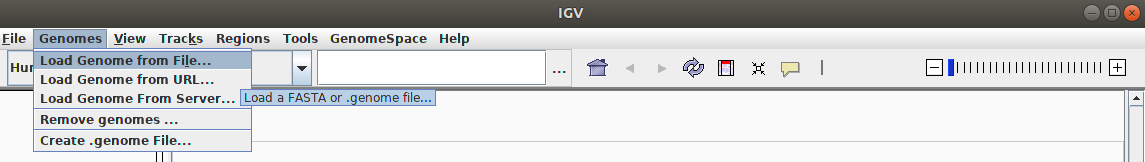
\includegraphics{images/load-yeast-ref.png}
\caption{Loading the yeast reference genome}
\end{figure}

    \begin{figure}
\centering
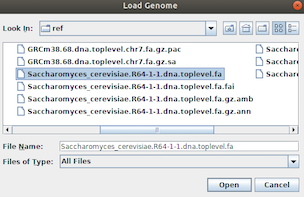
\includegraphics{images/yeast-ref-dialog.png}
\caption{Loading the yeast reference genome from a file}
\end{figure}

    \hypertarget{load-the-alignment}{%
\subsubsection{Load the alignment}\label{load-the-alignment}}

\textbf{To load the merged BAM file, on the top menu bar go to '
\textit{File --\textgreater{} Load from File\ldots{}} ' and select the
library BAM file that you created in the previous step.}

    \begin{figure}
\centering
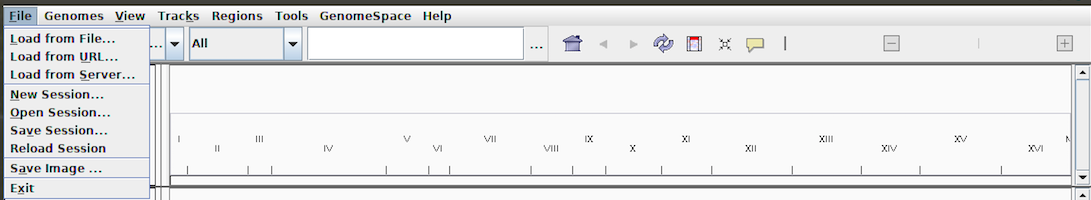
\includegraphics{images/load-yeast-bam.png}
\caption{Loading the yeast alignment"}
\end{figure}

    \begin{figure}
\centering
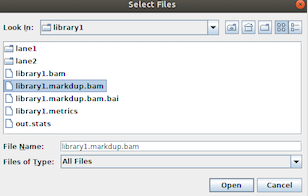
\includegraphics{images/yeast-bam-dialog.png}
\caption{Loading the yeast alignment}
\end{figure}

    \hypertarget{exercises}{%
\subsection{Exercises}\label{exercises}}

\begin{enumerate}
\def\labelenumi{\arabic{enumi}.}
\item
  Go to Chromosome IV and position 764,292. (\textbf{Hint: use the
  navigation bar across the top})
\item
  What is the reference base at this position?
\item
  Do the reads agree with the reference base?
\item
  What about the adjacent position (IV:764,293)? What is the reference
  base at this position? Is it supported by the reads?
\item
  Go to Chromosome IV and position 766,589.
\item
  What sort of mutation are the alignments indicating might be present?
\item
  Go to Chromosome IV and position 770,137 using the navigation bar
  across the top.
\item
  What sort of mutation are the alignments indicating might be present?
  Is there anything in the flanking sequence of the reference genome
  that might make you suspicious about this mutation?
\item
  Convert the BAM file to a CRAM file
\end{enumerate}

    You have reached the end of the Read Alignment tutorial.


    % Add a bibliography block to the postdoc



\end{document}
